\chapter{Automatic Metadata Extraction and Update}
\graphicspath{{figs/04-extraction-update/}}

As we have an application ready to receive and display metadata, it is now crutial to turn the attention to extracting metadata from CDM databases, which contain the actual data, allowing, then, to update the data stored on applications such as the MONTRA framework.

\section{Requirement Analysis}

%\begin{itemize}
%    \item nem sempre vamos ter acesso direto à base de dados
%        \item melhor optar por uma opção em que o tal agente apenas está à escuta de ficheiros num diretorio especifico
%    \item Comunicação com os agentes pode ser necessario para obter feadback. no entanto, segundo a literatura, ter portas aberta não é algo que devemos ter de pedir aos data owners, pois pode implicar alterações na sua firewal e afins.
%    \item existe a possiblidade de criar uma solução p2p, no entanto podemos estar a colocar responsabilidades nos agentes que os data owners podem não querer ter. uma melhor aproximação para garantir que a solução é mais apropriada para os data owners é uma entidade central que se encarrega das várias tarefas da rede.
%    \item o cargo do agente passa a ser apenas ler dados e enviar para um entidade central
%    \item data might not come in the desired format. need to transform
%    \item application might not want all the data extracted from a database. need to filter
%\end{itemize}

When we enter the realm of accessing an institution's sensitive data, some problems start to arise.
Not all data owners are willing to, or legally can't, provide direct access to their data.
When building this part of the system, we have to consider this and have several options available that use different levels of access and according to the demands of each specific data owner, use the most appropriate one.
In one end, a single solution could have full access to the data, extracting the metadata directly from the original data.
At the other end of the scale, the burden of extracting data is removed from us and the system is dependent on the data owner providing the metadata and only then the system processes the metadata.
Having several options for different access levels is more flexible, however, it requires maintaining several tools which are not reliable.
A more appropriate alternative is to have a single option, that is designed considering the most strict access to the data, however, we still need to provide a tool to extract the metadata.
The only difference is that we are not the ones executing it.

As the extracting tool has direct access to the data, using an existing and widely known tool is a must, so data owners are inclined to use it.
Additionally, making fewer to no changes is preferable to ensure that data owners don't discard the tool because they don't trust the changes.

\begin{figure}[h]
    \center
    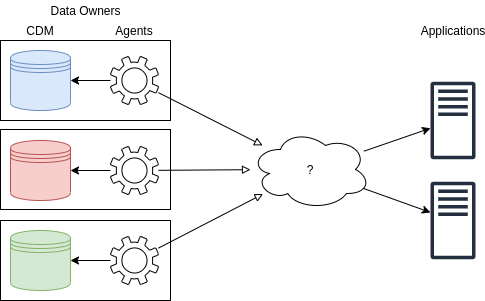
\includegraphics[width=.6\textwidth]{overall-arch}
    \caption{High-level architecture of the extraction and update process.}
    \label{fig:overall-arch}
\end{figure}

In figure \ref{fig:overall-arch} is presented the overall architecture of the system, where the agent is the tool in charge of parsing the metadata provided by the data owner, which is then sent to the applications.
Regarding this last point, there needs to be a way for the data to go from the agents to the applications.
One ambitious solution is to create a decentralized peer-to-peer network of agents, avoiding developing a central unit.
In such solution, the agents are in charge of managing and sending the data to the applications.
However, data owners might not want to spend their hardware resources to maintain a network.
Since the agents are executed on the data owner's system, they should do only the required and minimal functionality, spending the few resources as possible.

A more executable solution is to have an intermediate component that receives the metadata from the agents and then distributes that data across the applications, following a centralized architecture as it is presented in figure \ref{fig:new-overall-arch}.

\begin{figure}[h]
    \center
    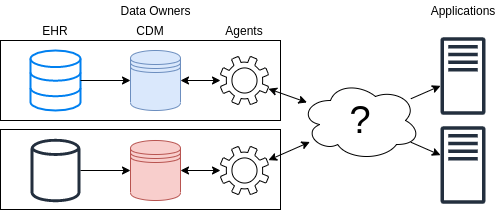
\includegraphics[width=.6\textwidth]{new-overall-arch}
    \caption{High-level architecture of the extraction and update process, with a centralized approach.}
    \label{fig:new-overall-arch}
\end{figure}

This centralized component will be used to manage the data and the applications to where such has to be sent.
However, it is also important that it provides feedback on the state of the system, such as how the data is flowing in the system, which applications received which data, and which databases sent data into the system.

% em cima digo que percicasos de um componente intermediario. mais á frente vou dizer que percisamos um componente intermediario entre o kafka e as aplicações. coisas diferentes

On the applications side, there are other important factors to consider before going forward on implementing the intermediary component mentioned before.
First, the \gls{api}s of different applications expect the metadata in distinct arrangements.
A way out of this would be to specify a set of endpoints that each application had to implement, yet that would lead the applications to have two sets of endpoints that do the same thing.
On the other side, making a flexible option, where the requests where the data is sent are customizable, would be more appealing for the target applications, which would not have to make any changes.
Second, not all applications require all metadata data that is extracted from a database.
Some use all the data, others only need a value of such data.

\subsection{Functional Requirements}

\begin{enumerate}
    % extraction tool
    \item The extraction tool used should either be one already built and

    % agents
    \item The agents muts not have direct access to the data

        \begin{list}{}{}
            \item This option assumes the least amount of access to the user's data so data owners are receptive to allow agents to be ran on their local deployments.
                This will require that an agent has access to at least a shared storage where agents check for new writes and data owners post their extracted metadata.
        \end{list}

    % central unit
    \item The central component must allow to register new databases

        \begin{list}{}{}
            \item cenas
        \end{list}

    \item The central component must allow to check if databases are active

        \begin{list}{}{}
            \item
        \end{list}

    \item The central component must allow check the amount of data a database has sent

        \begin{list}{}{}
            \item
        \end{list}

    \item The central components must alow to filter and select portions of the received data

        \begin{list}{}{}
            \item
        \end{list}

    % aplications
    \item The central components must allow to register new applicaitons

        \begin{list}{}{}
            \item
        \end{list}

    \item The format of the data when being received by aplications must be cutomizable

        \begin{list}{}{}
            \item
        \end{list}

    \item The central components must allow to see the amounts of data that was sent to the aplications

        \begin{list}{}{}
            \item
        \end{list}

\end{enumerate}

\subsection{Non-Functional Requirements}

\begin{enumerate}
    \item Easily deployable

        \begin{list}{}{}
            \item the instalations of the agents by the admin of data owner's data center should be a smoth process
        \end{list}

    \item agents should spend few resources

        \begin{list}{}{}
            \item
        \end{list}

    \item Scallable

        \begin{list}{}{}
            \item
        \end{list}

    \item Micro service architecture

        \begin{list}{}{}
            \item As more databases are connected to the network, the system should allow to increase resources so that is processes faster
        \end{list}

    \item Agents should do only the necessary

        \begin{list}{}{}
            \item The system should be composed by simple and replacable components that deal with well defined tasks
        \end{list}

\end{enumerate}

\subsection{Use Cases}

actors:
- data owners
install agent
stop agent

admin
- all other things

\section{Extraction}

\begin{itemize}
    \item a ideia geral em mente
    \item diagrama high-level do data flow
\end{itemize}

\subsection{ACHILLES}
\begin{itemize}
    \item organização interna
    \item implementado em R
    \item diferentes maneiras de exportação (json, csv ou diramente para db)
    \item a query for each analaysis
    \item Catalogue Export
\end{itemize}

\subsection{Asynchronous Message Systems}

\subsubsection{RabbitMQ}

\subsubsection{Kafka}


\subsection{Kafka Source Connectors}
\begin{itemize}
    \item fetch from files
    \item falar nas varias opcoes
    \item o que eu escolhi da feedback de quando todos os records estão kafka e quantos records foram escritos
\end{itemize}

% ---

\subsection{agent final architecture}
\begin{enumerate}
    \item send data to kafka
    \item responde to health check messages
\end{enumerate}

\begin{figure}[h]
    \center
    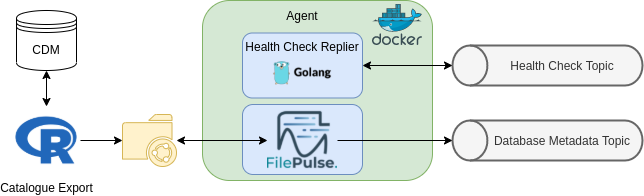
\includegraphics[width=\textwidth]{agent-architecture}
    \caption{agent arch}
    \label{fig:agent-architecture}
\end{figure}

\section{Publishing}

data is in kafka. what do we have to do to reach the applications

\begin{itemize}
    \item need to send custom data on a CUSTOM FORMAT to a custom REST endpoint
    \item Kafka Sink Connectors (The target REST API is not customizable, such as the data format ) - need for a sender application
    \item No known end on kafka topics/streams - require some management on top of kafka
\end{itemize}

\section{Network Manager}  % change name
\begin{itemize}
    \item centralized entity
    \item transforms the data to the required format
    \item sends to the specific application's endpoint
    \item 4 components
\end{itemize}

\subsection{Pipelines Workers}
\begin{itemize}
    \item select and filter the data comming from the databses
    \item only process data of a single database at a time. handling multiple is the same is hard to handle and hard to scale
    \item scalable: several pipeline worker applications
\end{itemize}
\subsection{Orchestrator}
\begin{itemize}
    \item To ensure multiple records of multiple databases are not processes at the same time, this component redirects the data from databases to the pipelines workers preventing the previous problem
\end{itemize}
\subsection{Sender}
\begin{itemize}
    \item sends/publishes the data resulting from the pipelines, to the application's endpoints
\end{itemize}
\subsection{Admin Dashboard}
\begin{itemize}
    \item manage the whole thing
    \item Allows to create new pipelines and add aplications
\end{itemize}

\section{Network Data Flow}
\begin{itemize}
    \item Evaluation?
    \item step by step
    \item number of topics involved
\end{itemize}
